\documentclass{standalone}

\usepackage{pgfplots}
\usetikzlibrary{calc}
\usepgfplotslibrary{groupplots}
\begin{document}
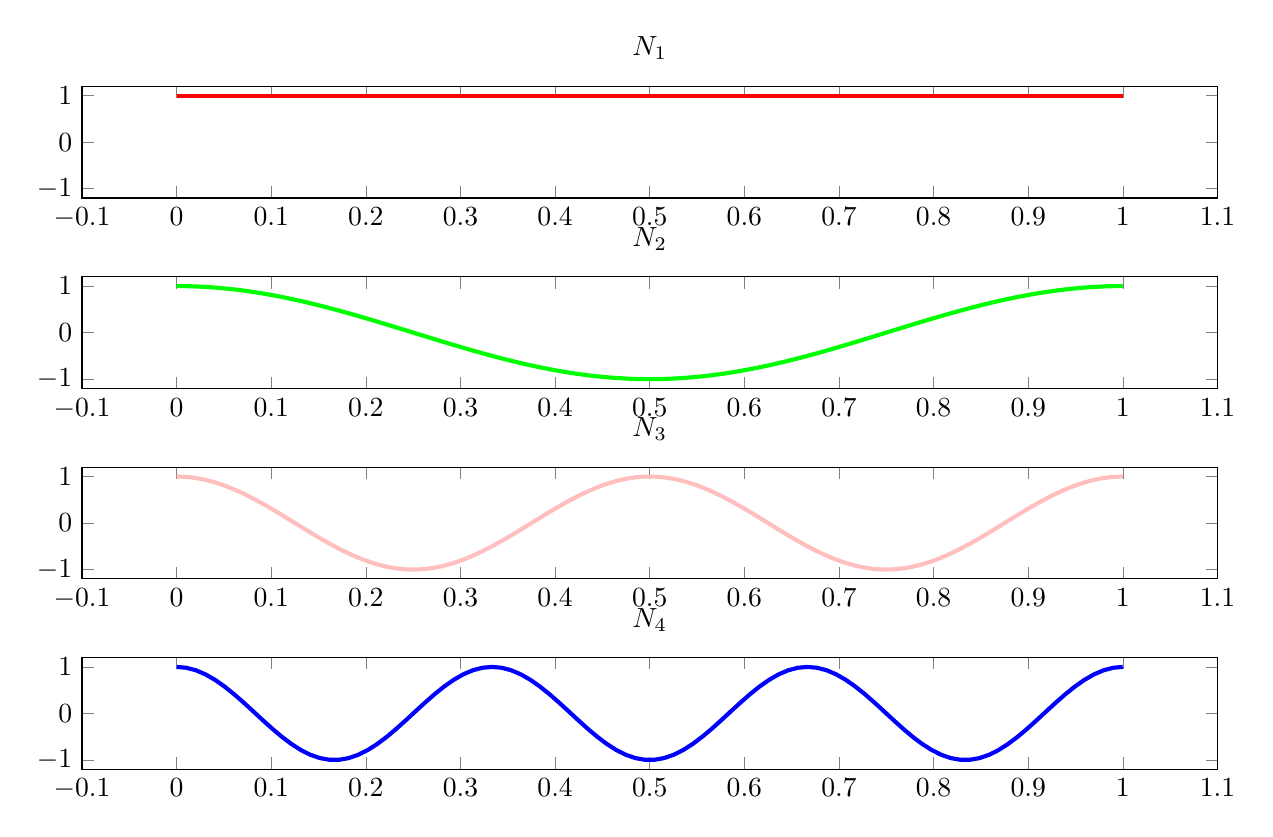
\begin{tikzpicture}
  \begin{groupplot}[group style={group size=1 by 4},height=3cm,width=16cm,trig format plots=rad,ymin=-1.2, ymax=1.2,]
    \nextgroupplot[title=$N_1$]
    \addplot [domain=0:1,color=red,samples=100,mark=none, line width = 1.5]{cos(2*pi*0)};
    \nextgroupplot[title=$N_2$]
    \addplot [domain=0:1,color=green,samples=100,mark=none, line width = 1.5]{cos(2*pi*x)};
    \nextgroupplot[title=$N_3$]
    \addplot [domain=0:1,color=pink,samples=100,mark=none, line width = 1.5]{cos(4*pi*x)};
    \nextgroupplot[title=$N_4$]
    \addplot [domain=0:1,color=blue,samples=100,mark=none, line width = 1.5]{cos(6*pi*x)};
  \end{groupplot}
% \node (title) at ($(group c1r1.center)!0.5!(group c1r2.center)+(0,2cm)$) {THE Title};
\end{tikzpicture}
\end{document}